\documentclass[a4paper, 10pt, conference]{IEEEtran}
\usepackage{enumitem}
\usepackage{graphicx,float}
\usepackage{subcaption}

\newcommand{\head}[1]{\textnormal{\textbf{#1}}}

\title{Outcome Prediction of ODI Cricket Matches using Decision Trees and MLP Networks}

\author{
\IEEEauthorblockN{\IEEEauthorrefmark{1}Rajeev Kumar,\IEEEauthorrefmark{2}Jalaz Kumar}
\IEEEauthorblockA{
\IEEEauthorrefmark{1}Assistant Professor,\IEEEauthorrefmark{2}Student\\
Department of Computer Science and Engineering\\
National Institute of Technology Hamirpur, India\\
\IEEEauthorrefmark{1}rajeev@nith.ac.in,\IEEEauthorrefmark{2}jalazkumar1208@gmail.com}}

\begin{document}

\maketitle
\thispagestyle{empty}
\pagestyle{empty}


%%%%%%%%%%%%%%%%%%%%%%%%%%%%%%%%%%%%%%%%%%%%%%%%%%%%%%%%%%%%%%%%%%%%%%%%%%%%%%%%
\begin{abstract}

Applications of Machine Learning supplemented with Data Mining Techniques has become a hot topic for research worldwide, Sports Analytics is no exception though. Cricket is one of the most popular sports in Australia, Caribbean, UK \& South Asian Nations with a net fan base of around 2.5 billion. The game has tremendous spectator support in more than 100 nations and the masses show great interest in predicting the game outcomes. There are lots of pre-game and in-game attributes which decides the outcome of a cricket match. Pre-game attributes like the venue, past track-records, Innings(First/Second), team strength etc. and the various in-game attributes like Toss, run rate, wickets remaining, strike rate etc. influence the result of a match in a predominant manner. In our study, we have used 2 different ML approaches, Decision Trees \& MultiLayer Perceptron Network, to analyse the effect produced on the outcome of a Cricket match due to these varied factors. Based on these results, We have designed CricAI: Cricket Match Outcome Prediction System. Our designed tool takes into consideration the pre-game attributes like the ground, venue (home, away, neutral) \& innings (first/second) for predicting the final result of given match.


Keywords: Decision Tree Classifier, Multi Layer Perceptron Classifier, Features, Performance Measures

\end{abstract}


%%%%%%%%%%%%%%%%%%%%%%%%%%%%%%%%%%%%%%%%%%%%%%%%%%%%%%%%%%%%%%%%%%%%%%%%%%%%%%%%
\section{INTRODUCTION}

Cricket is basically a bat and ball game which is played between 2 teams having 11 players each. Each team comes to bat and has a single inning in which it seeks to score as many runs as possible, while the other team fields. The innings ends when the total quota of deliveries, which depends on game format has turned up, or the 10 batsmen have been dismissed, whichever comes first. The prime objective is to score more runs \& thus Runs are the decisive factor.

Game of Cricket is highly unpredictable in nature. Until the very last moment, it is difficult to make accurate predictions about the game. Various natural factors affecting the game output, huge betting market and enormous media coverage have given strong incentives to model this game from the Machine Learning Perspective.

International Cricket Council (ICC) is the governing body which decides the rules of Cricket.

There are 3 widely accepted formats of Cricket on International level - T20 match, One Day Internationals and Test match. The scheduled duration of the game is the prime difference between these three formats, which directly modifies the number of deliveries each team got to play in their respective innings.

Test cricket format is the longest one and is considered as the highest standard of the game. Match duration is five days in which each team get to play 2 innings each. A standard day of test cricket match comprises of 3 sessions each of 2 hours.

One Day International i.e. ODI format is in limited overs, where each team faces 300 deliveries(50 overs). Generaly, ODI match falls in any of the 2 categories: Day or Day-Night Match

T20 is the shortest internationally recognized format of this game, where each team innings consist of 20 overs. This is more of an "explosive" and more "athletic" than the other two formats.

Our study is focused on the most popular format of Cricket, One Day Internationals or the ODIs. The outcome of One Day Internationals is influenced by a varied no. of features and can be predicted like all other games. We need to find the best attributes or factors that influence the match outcome. For our analysis, we have considered the factors used by [1] and [2], which are proven to have a substantial impact on the match outcome. The factors considered for analysis include:

\begin{description}
  \item[$\bullet$ Teams Past Performance:] This factor captures the historic outcomes of all the matches played between the teams.
  \item[$\bullet$ Ground:] This plays a vital role as teams have great track records on particular grounds and carry psychological superiority over the other.
  \item[$\bullet$ Innings:] This factor determines which team batted first \& which batted second.
  \item[$\bullet$ Home Game Advantage:] This is achieved by using Venue feature, which determines whether a particular ground is home/away/neutral for each of the playing teams.
\end{description}

Both of our classifiers are trained on the basis of these factors. For predicting the final result of Cricket matches we have used 2 supervised classification techniques - Decision Trees and Multi-Layer Perceptron Networks. Comparative study is conducted between both the classifiers and final results are summarized in this paper. 

We then built a Desktop App called CricAI based on emerged results, which can be used for predicting the final outcome of any Cricket match given the appropriate features as the inputs. This software of ours can be of real value to the cricketers, support staff of teams and the cricket governing bodies for analysing the future course of game well in advance and working accordingly so as to maximize the victory chances.

Since, we need to deal with multiple independent attributes, therefore clustering them after finding similarity patterns doesn't seem feasible, due to which Clustering doesn't make any reasonable contribution to our research. 

The rest of this paper is organised as follows. Section 2 explains the approach we have taken into account for the proposed analysis. Section 3 deals with the comparative analysis of both the classifiers used. Section 4 presents the other related works in this domain. Section 5 gives the conclusions and the future scope associated with this approach.

%%%%%%%%%%%%%%%%%%%%%%%%%%%%%%%%%%%%%%%%%%%%%%%%%%%%%%%%%%%%%%%%%%%%%%%%%%%%%%%%%%%%%

\section{APPROACH FOR ANALYSIS}

\subsection{Data Collection}

Data was extracted from [3] by running a scraping script in a justified manner, sending 1 request per second.
\begin{table}[h!]
  \begin{center}
    \caption{Scrapped Dataset Format}
    \label{tab:table1}
    \begin{tabular}{cccccc} 
      \textbf{Match Id} & \textbf{Team 1} & \textbf{Team 2} & \textbf{Winner} & \textbf{Margin} & \textbf{Ground}\\
      \hline
      ODI \#1 & Australia & England & Australia & 5 wickets & Melbourne\\
      ODI \#2 & England & Australia & England & 6 wickets & Manchester\\
      ODI \#3 & England & Australia & Australia & 5 wickets & Lord's\\
    \end{tabular}
  \end{center}
\end{table}

Dataset comprises of all the ODI matches from Jan 5, 1971, to Oct 29, 2017. A total of 3933 ODI match results were scrapped. The collected dataset was subjected to cleaning process where some of the matches were deleted from the analysis. Since it's not possible to foresee the impact of nature on cricket, matches which either ended up in a tie/draw or interrupted by rain, were being removed from the dataset. Matches of Special teams like World XI, Asia XI \& Africa XI were also removed.

We also further replicated our dataset two times by swapping the team positions i.e. A game between Team 1: India and Team 2: Sri Lanka was also replicated as Team 1: Sri Lanka and Team 2: India. For further making the dataset suitable for input to the various Machine Learning Classifier Models, we converted the continuous dataset into a categorical dataset, using dummy variables.

\textbf{Innings Feature} was determined by first translating Column: \textit{Margin} into Column: \textit{Winner Innings} using:\\
\indent \indent $\cdot$ Win by Wickets  $\Longrightarrow$  Winner Innings: 2\\
\indent \indent $\cdot$ Win by Runs \indent $ \Longrightarrow$  Winner Innings: 1
\\Further, Using Column: \textit{Winner} and the generated  Column: \textit{Winner Innings}, we aquired the innings of each team per match.

\textbf{Venue Feature} was determined by using Column: \textit{Winner} and Scrapped dataframe from [3] which provided the names of cricket grounds in all countries. Combining both of these, Column: \textit{Host Country} was generated, which was used to get venue of a match with respect to both the teams.

The dataset was saved in comma separated format. We used a total of 7494 match records for our analytical study which was further divided into the testing and training data.
\\$\star$ Training Dataset Size: 5620
\\$\star$ Testing Dataset Size: 1874

\subsection{MultiLayer Perceptron Networks}
MLP Network is a type of supervised learning algorithm which learns a function \[ f(.): R^{n} \rightarrow R^{t} \] by using some training dataset, where \textit{t} is the total number of output units and \textit{n} is the total number of input units. Given features set \textit{X = $x_{1}$, $x_{2}$, ..., $x_{m}$} and a target \textit{y},  MLP Network can be trained to be a non-linear function approximator for classification as well as regression. The core difference between MLP Networks and Logistic regression is in the former one there can be hiddem layers, which are actually one or more nonlinear layers. Fig 1. shows a Multi-layer Perceptron Network with only 1 hidden layer.
\begin{figure}
  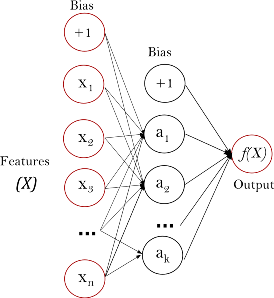
\includegraphics[width=\linewidth]{MLP.png}
  \caption{Multilayer Perceptron Network}
  \label{fig:mlp}
\end{figure}

Input Layer is the leftmost layer representing the input features, consists of a set of neurons. \[ {x_{i}|x_{1},x_{2},\ldots,x_{m}} \]Values from the previous layers are transformed using weighted linear summation by the neurons of the Hidden Layer, \[ w_{1}x_{1} + w_{2}x_{2} + \ldots + w_{m}x_{m} \]
followed by a non-linear activation function acting on its output. The last hidden layer further transfers these values towards the output layer which transforms these intermediate values into the final output values.

MLPClassifier [4] is implemented using a multi-layer perceptron (MLP) algorithm in which Backpropagation is used for training. More precisely, some form of gradient descent is actually used to train the dataset, and such gradient values are computed using Backpropagation.

MLP trains using two input arrays: array \textbf{X} of size(n\_samples, n\_features); and array \textbf{y} of size (n\_samples). All feature vectors comprises of the training samples are held in \textbf{X} \& the target values(class labels) for respective training samples are held in \textbf{y}.

Currently, Only the Cross-Entropy loss function is supported by the MLPClassifier [4], using which we can derive the estimated probabilities by running predict\_proba function. MLPClassifier also supports multi-class classification in which any input feature set can belong to more than one class which makes it quite suitable for our approach. \\

\textbf{Advantages:}\\
\indent $\ast$ MLP Networks are capable to run all types of non-linear models.\\
\indent $\ast$ MLPClassifier uses Backpropagation so, it continously learns and improvize itself.\\
\indent $\ast$ MLP Networks are capable to learn \& train in real\-time using partial fitting property.\\

\textbf{Disadvantages:}\\
\indent $\ast$ MLP Networks are highly sensitive for feature scaling.\\
\indent $\ast$ It uses a black box model, interpretation of results may become difficult.\\
\indent $\ast$ MLP Networks requires a large number of hyperparameters \& thus proper tuning of the number of epochs, hidden neurons and layers is required.

\subsection{Decision Trees}
Decision Trees are also a type of Supervised Machine Learning techniques where according to a certain parameter input training data is continuously split up. Any decision tree can be explained using two of its entities, decision nodes and leaf nodes. The leaves denote the final outcomes or the overall decisions made and our data is split using some entropy calculation at the decision nodes.
Decision Trees (DTs) can be used for both classification as well as regression problems. The entire goal is to create a supervised model which can predict the value of any input target variable by making use of the prominent decision rules formulated from the training dataset features.
\begin{figure}
  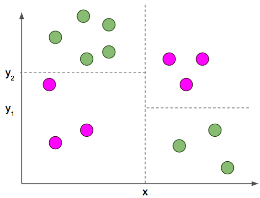
\includegraphics[width=\linewidth]{DecisionTree.png}
  \caption{Decision Tree}
  \label{fig:dt}
\end{figure}

Given, \textit{$x_{i}\epsilon$ $R^{n}$, i=1,..., l} are the training vectors and \textit{y$\epsilon$ $R^{l}$} is the target vector, recursive partitioning of entire dataset is done by the decision tree such that data samples with same target labels get in a single group. Let \textit{Q} represents the data at node \textit{m}. For each candidate node, partition the data into \textit{$Q_{left}$($\theta$)} and \textit{$Q_{right}$($\theta$)} subsets using split \textit{$\theta$ \= (j,$t_{m}$)} which consists of a feature \textit{j} and threshold \textit{$t_{m}$},
\[ Q_{left}(\theta) = (x,y)|x_{j}<=t_{m}
\]
\[ Q_{right}(\theta) = Q/Q_{left}(\theta)
\]

An impurity function \textit{H()} is used to compute the impurity at \textit{m} , whose choice depends on the task under consideration (regression or classification).
\[ G(Q,\theta) = \frac{n_{left}}{N_{m}}H(Q_{left}(\theta)) + \frac{n_{right}}{N_{m}}H(Q_{right}(\theta))
\]
Select the parameters that minimises the impurity
\[ \theta^{\ast} = arg min_{\theta}G(Q,\theta)
\]
Continue partitioning recursively for the subsets \textit{$Q_{left}(\theta^{\ast})$} and \textit{$Q_{right}(\theta^{\ast})$} until the maximum allowable depth is reached, \textit{$N_{m}< min_{samples}$} or \textit{$N_{m}$}=1.
\\

\textbf{Advantages:}\\
\indent $\ast$ Decision Trees are simple enough to understand, interpret its outcome and visualize the results.\\
\indent $\ast$ Able to handle both numeric as well as categorical data and also multi-output problems.\\\
\indent $\ast$ The White box model is followed up. If some situation is observable in the model, then its explanation is easily explained using the logic of Boolean Algebra.\\

\textbf{Disadvantages:}\\
\indent $\ast$ Sometimes complex trees are created which are not able to generalize the data well. Decision Trees are prone to Over-fitting.\\
\indent $\ast$ Decision trees are usually very unstable and even small modifications in the data might lead to an entirely different tree being generated.\\
\indent $\ast$ For the cases, where some classes dominate creation of biased Decision Tree takes place.\\

%%%%%%%%%%%%%%%%%%%%%%%%%%%%%%%%%%%%%%%%%%%%%%%%%%%%%%%%%%%%%%%%%%%%%%%%%%%%%%%%%%%%%%%

\section{RESULTS AND OBSERVATIONS}

\subsection{Performance Measures}
To evaluate classifier performance in a well effective manner, we need to define the performance measure. Efficiency and goodness of any classifier is measured by the various defined performance measures which is itself a single index.

We have performed a comparative analysis of our classifiers considering the following performance measures: 

\textbf{Accuracy Score:}
 This compares the actual outcomes with the predicted outcomes of our classifier for a given input dataset. For best Accuracy Score, the set of actual true labels in testing dataset must match the corresponding set of predicted labels.

For measuring the success of our prediction, Precision-Recall is a useful index. In information retrieval, result relevancy is measured using precision, while recall is a measure of the total number of truly relevant results which were returned.

\textbf{Precision Score:}
This is defined as the number of true positives $(T_{p})$ divided by the number of true positives plus the number of false positives $(F_{p})$
\[ P = \frac{T_{p}}{T_{p}+F_{p}}\]
The precision is the ability of the classification model for not labelling a negative sample as a positive one. Best value: 1 and Worst value: 0. 

\textbf{Recall Score:}
This is defined as the number of true positives $(T_{p})$ divided by the number of true positives plus the number of false negatives $(F_{n})$
\[ P = \frac{T_{p}}{T_{p}+F_{n}}\]
The recall is the ability of the classification model of finding all the possible positive samples. Best value: 1 and Worst value: 0.

\textbf{F1 Score:}
This is defined as the interpretation of a weighted average of the recall score and precision score of a classifier. Numerically, it is equal to the harmonic mean of the precision-score and recall-score.
\[ F1 = 2 \frac{P*R}{P+R}
\]
It is also known as the F-measure or balanced F-score. Both precision and recall have an equal relative contribution to the F1 score.

\textbf{Average Precision Score:}
This is defined as the weighted mean of precisions achieved at each threshold value, summarized using precision-recall curve:
\[ AP = \Sigma_{k}(R_{k}-R_{k-1})P_{k}\]
where \textit{$R_{k}$} and \textit{$P_{k}$} are the recall and precision at the \textit{$k^{th}$} threshold.

\subsection{Comparative Analysis}
\textbf{Accuracy Score:}
\begin{figure}[h!]
  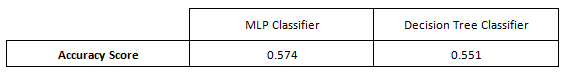
\includegraphics[width=\linewidth]{ModelScore.png}
  \label{fig:scoremodel}
\end{figure}

\textbf{Observation:}
We selected 3 teams: India, Australia and Pakistan randomly and separated the match records of these 3 teams to obtain the performance measure for them separately.
\begin{figure}[h!]
  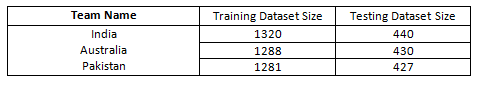
\includegraphics[width=\linewidth]{DatasetTeam.png}
  \label{fig:teamdata}
\end{figure}

\begin{figure}[h!]
  \centering
  \begin{subfigure}[b]{0.4\linewidth}
    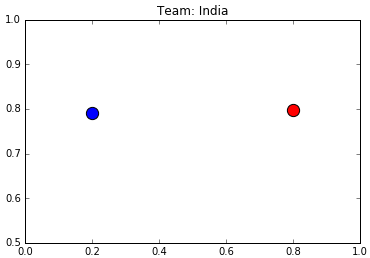
\includegraphics[width=\linewidth]{MLPCLF_India.png}
    \caption{P = 0.791, R = 0.797}
  \end{subfigure}
  \begin{subfigure}[b]{0.4\linewidth}
    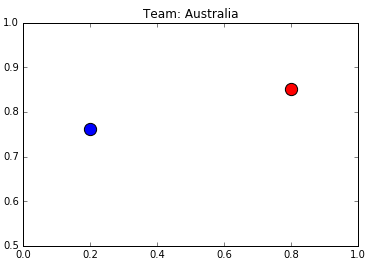
\includegraphics[width=\linewidth]{MLPCLF_Australia.png}
    \caption{P = 0.760, R = 0.850}
  \end{subfigure}
  \begin{subfigure}[b]{0.4\linewidth}
    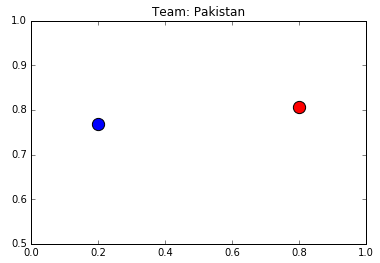
\includegraphics[width=\linewidth]{MLPCLF_Pakistan.png}
    \caption{P = 0.767, R = 0.806}
  \end{subfigure}
  \caption{Precision-Recall Scatter Plot for MLP Classifier.}
  \label{fig:mlpclfPlots}
\end{figure}

\begin{figure}[h!]
  \centering
  \begin{subfigure}[b]{0.4\linewidth}
    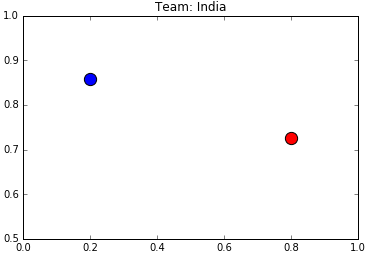
\includegraphics[width=\linewidth]{DTCLF_India.png}
    \caption{P = 0.859, R = 0.726}
  \end{subfigure}
  \begin{subfigure}[b]{0.4\linewidth}
    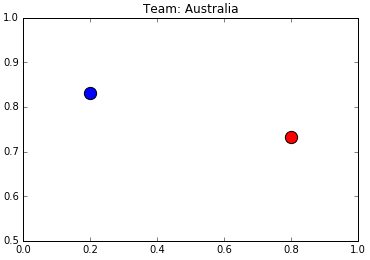
\includegraphics[width=\linewidth]{DTCLF_Australia.png}
    \caption{P = 0.830, R = 0.733}
  \end{subfigure}
  \begin{subfigure}[b]{0.4\linewidth}
    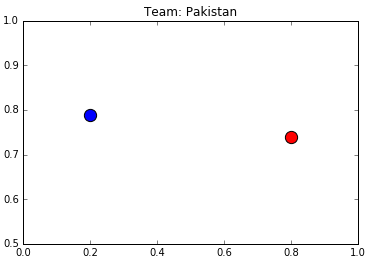
\includegraphics[width=\linewidth]{DTCLF_Pakistan.png}
    \caption{P = 0.789, R = 0.739}
  \end{subfigure}
  \caption{Precision-Recall Scatter Plot for DT Classifier.}
  \label{fig:dtclfPlots}
\end{figure}

\begin{figure}[h!]
  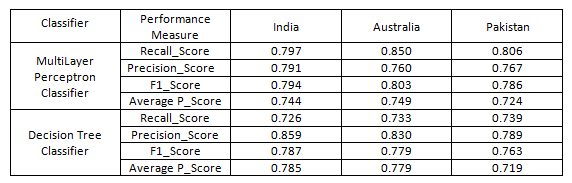
\includegraphics[width=\linewidth]{TeamScore.png}
  \label{fig:results}
\end{figure}

%%%%%%%%%%%%%%%%%%%%%%%%%%%%%%%%%%%%%%%%%%%%%%%%%%%%%%%%%%%%%%%%%%%%%%%%%%%%%%%%%%%%%%%

\section{RELATED WORK}
From our literature survey, we observed that game of cricket has very few machine learning related work done on it. Despite sharing numerous features with other sports like baseball, game of cricket is unique of its type and thus an independent analysis is required.

Statistical Approach is the base of majority of the analytical studies \& research done on cricket.

Prediction of the outcome of an in-progress game in one-day international cricket was conducted by Bailey and Clarke [5]. WASP(Winning and Score Predictor), 2012 is a product grounded on the theory of Dynamic Programming, by Dr Scott Brooker and Dr Seamus Hogan at the University of Canterbury in New Zealand.

Neeraj Pathak \& Hardik Wadhwa conducted a similar comparative analysis of match outcomes using the classification models: Support Vector Machines, Random Forests and Naive Bayes[6].Preeti Satao and Team predicted the score of cricket match using Clustering Techniques[7].

In Parag Shah, Mitesh Shah[8] and Amal Kaluarachchi, Aparna S. Varde[9], they explored the statistical significance of a range of factors \& game-attributes which explain the outcome of a cricket match. In particular, home crowd advantage, match type (day-night/day), past performance of the team against each other \& game plan (batting first or fielding first) were the key interests in their investigation.

Madan Gopal Jhanwar and Vikram Pudi used a supervised learning approach from some team composition perspective for predicting the result of an One Day International (ODI) cricket match. Their work suggested that one of the distinctive features for predicting the winner is the relative team strength of both the competing teams. Swetha and Saravanan.KN analysed the factors that cricket game depends on and decides Winning[1]. 

%%%%%%%%%%%%%%%%%%%%%%%%%%%%%%%%%%%%%%%%%%%%%%%%%%%%%%%%%%%%%%%%%%%%%%%%%%%%%%%%%%%%%%%

\section{CONCLUSION}

In our study, we performed a comparative analysis of the predictions generated by 2 different supervised classification models for the same input dataset. We are able to predict the final game outcomes using the pre-game attributes as the features of the dataset.

The major contributions of our study are:
\begin{description}
  \item$\bullet$ Comparative analysis of performance measure of two different supervised learning techniques. 
  \item$\bullet$ Analysing all the factors which strive to affect the final outcome of the game of cricket.
  \item$\bullet$ Design \& Development of a Prediction Desktop App which can be used to predict the chances of winning, using input attributes.
\end{description}

As future course of work, we plan to expand this analytical study more from the team composition perspective. Also, the relevance of considering 1980s match data equivalent to the 2017s match data also need to be analysed and worked upon. We can also apply our methodology and technique to predict the outcomes of games like hockey and football.
%%%%%%%%%%%%%%%%%%%%%%%%%%%%%%%%%%%%%%%%%%%%%%%%%%%%%%%%%%%%%%%%%%%%%%%%%%%%%%%%%%%%%%%

\section{ACKNOWLEDGMENT}

This research was supported by the Department of Computer Science and Engineering, NIT Hamirpur, India.

We are grateful to all our colleagues who provided support and insight which assisted us a lot in carrying out this research.
  
We also thank all of them for their worthy comments \& criticism on an earlier version, although any errors are our own and reputations of these esteemed persons should not be tarnished.

%%%%%%%%%%%%%%%%%%%%%%%%%%%%%%%%%%%%%%%%%%%%%%%%%%%%%%%%%%%%%%%%%%%%%%%%%%%%%%%%


\begin{thebibliography}{99}

\bibitem{c1} Swetha and Saravanan KN, "Analysis on Attributes Deciding Cricket Winning", International Research Journal of Engineering and Technology (IRJET), p-ISSN: 2395-0072, Volume: 04 Issue: 03 — March-2017
\bibitem{c2} Mehvish Khan and Riddhi Shah. "Role of External Factors on Outcome of a One Day International Cricket (ODI) Match and Predictive Analysis", International Journal of Advanced Research in Computer and Communication Engineering Vol. 4, Issue 6, June 2015.
\bibitem{c3} ESPN Cricinfo, http://www.stats.espncricinfo.com
\bibitem{c4} Scikit learn, http://scikit-learn.org/stable/index.html
\bibitem{c5} Bailey and Clarke, Journal of Sports Science and Medicine, 2006, Vol. 5, pp. 480487.
\bibitem{c6} Neeraj Pathak and Hardik Wadhwa,"Applications of modern classification techniques to predict the outcome of ODI Cricket". 2016 International Conference on Computational Science.
\bibitem{c7} "CRICKET SCORE PREDICTION SYSTEM (CSPS) USING CLUSTERING ALGORITHM", Preeti Satao, Ashutosh Tripathi, Jayesh Vankar, Bhavesh Vaje, Vinay Varekar.  International Journal Of Current Engineering and Scientific Research (IJCESR), 23940697, Volume-3, Issue-4, 2016.
\bibitem{c8} Parag Shah and Mitesh Shah, "Predicting ODI Cricket Result". Journal of Tourism, Hospitality and Sports, 2312-5179, Vol.5, 2015.
\bibitem{c9} Kaluarachchi, Amal, and S. Varde Aparna. "CricAI: A classification based tool to predict the outcome in ODI cricket." 2010 Fifth International Conference on Information and Automation for Sustainability. IEEE, 2010.
\bibitem{c10}  Madan Gopal Jhanwar and Vikram Pudi, "Predicting the Outcome of ODI Cricket Matches: A Team Composition Based Approach", European Conference on Machine Learning and Principles and Practice of Knowledge Discovery in Databases, Report No: IIIT/TR/2016/-1, Conference Center, Riva del Garda.

\end{thebibliography}

\end{document}
